\section{Data Processing}

Before any gestures can be predicted, the data must be prepared. There are two considerations for this. First, the preprocessing method must be fast and simple, as it needs to run with near zero latency on edge hardware (for example in a prosthetic hand). Second, the goal of using a deep neural network is to \emph{learn} robust features. Therefore, preprocessing methods must not profoundly alter the data, they must be simple methods which contain the maximum amount of available information. To start, the data (collected at 200 Hz), is sampled in time windows of 260 milliseconds (or 52 time steps), following the precedent set in \cite{primary}. One window of raw data can be seen in \autoref{fig:raw}.

\begin{figure}[h]
\caption{One window of sEMG data. The amplitude represents unitless motor activity potential, while the x axis represents the passage of time}
\label{fig:raw}
    \centering
    \def\svgwidth{0.7\columnwidth}
    \input{fig/raw.pdf_tex}
\end{figure}

This raw data represents what is collected by the two MYO armbands. Each armband collects 8-channel signal across the arm at 200 Hz. To remove any powerline interference, the armband collects the data with a notch filter which automatically removes the effects of large nearby electronics (such as power lines). The next step taken to make the signal more rich in information was to rectify (in layman's terms, take the absolute value of) the signal. In \cite{rectif}, it was shown that rectification significantly increased the availability of information pertaining to the  firing rate (temporal activity and pattern) of the motor units producing the signal. This means that rectification of the sEMG makes the information which allows for the learning of a pattern or feature which maps to a specific gesture more readily available.
\par After making the information denser, the next important preprocessing step is to make the information clearer. This is done in two ways. First, the packet of rectified signal is passed through a high pass Butterworth filter at 20 Hz. This removes any low frequency artifacts (aliases), which obscure the relevant signal. Finally, the data is passed through a moving average filter, which makes it more evident when the muscles are going through different periods of activity \cite{humancom}. The results of this preprocessing can be seen in \autoref{fig:proc}.
\begin{figure}[H]
\caption{One window of sEMG data. The amplitude represents unitless motor activity potential, while the x axis represents the passage of time. This data has been first rectified, then passed through a high pass filter, then passed through a 15-timestep moving average filter.}
\label{fig:proc}
    \centering
    \def\svgwidth{0.7\columnwidth}
    \input{fig/preprocessed.pdf_tex}
\end{figure}

\subsection{Data Augmentation}

One of the great challenges of deep learning, even with barely processed data, is its incredible capacity to overfit. In order to learn more robust mappings, without collecting a significantly larger amount of data, synthetic data must be generated, in order to prevent the deep learning algorithm from simply memorizing the training data. In this study, a novel data augmentation technique was employed, as seen in \autoref{fig:aug}. The methodology for the data augmentation is a simple random sample of a spectrum of different signal to noise ratios (SNR). A processed series is fed into the augmenter, and then random noise, at a given signal to noise ratio in magnitude is added. The signal to noise ratio for a realization is calculated at random as well, with linearly increasing likelihood as SNR increases. This allows the model to be trained for an extended period, without ever seeing the same observation twice.


\begin{figure}[H]
\caption{%
Data augmentation scheme, highlighted on a single channel of a single sample. Brighter realizations are more likely than dim ones.
}
\label{fig:aug}
\begin{center}
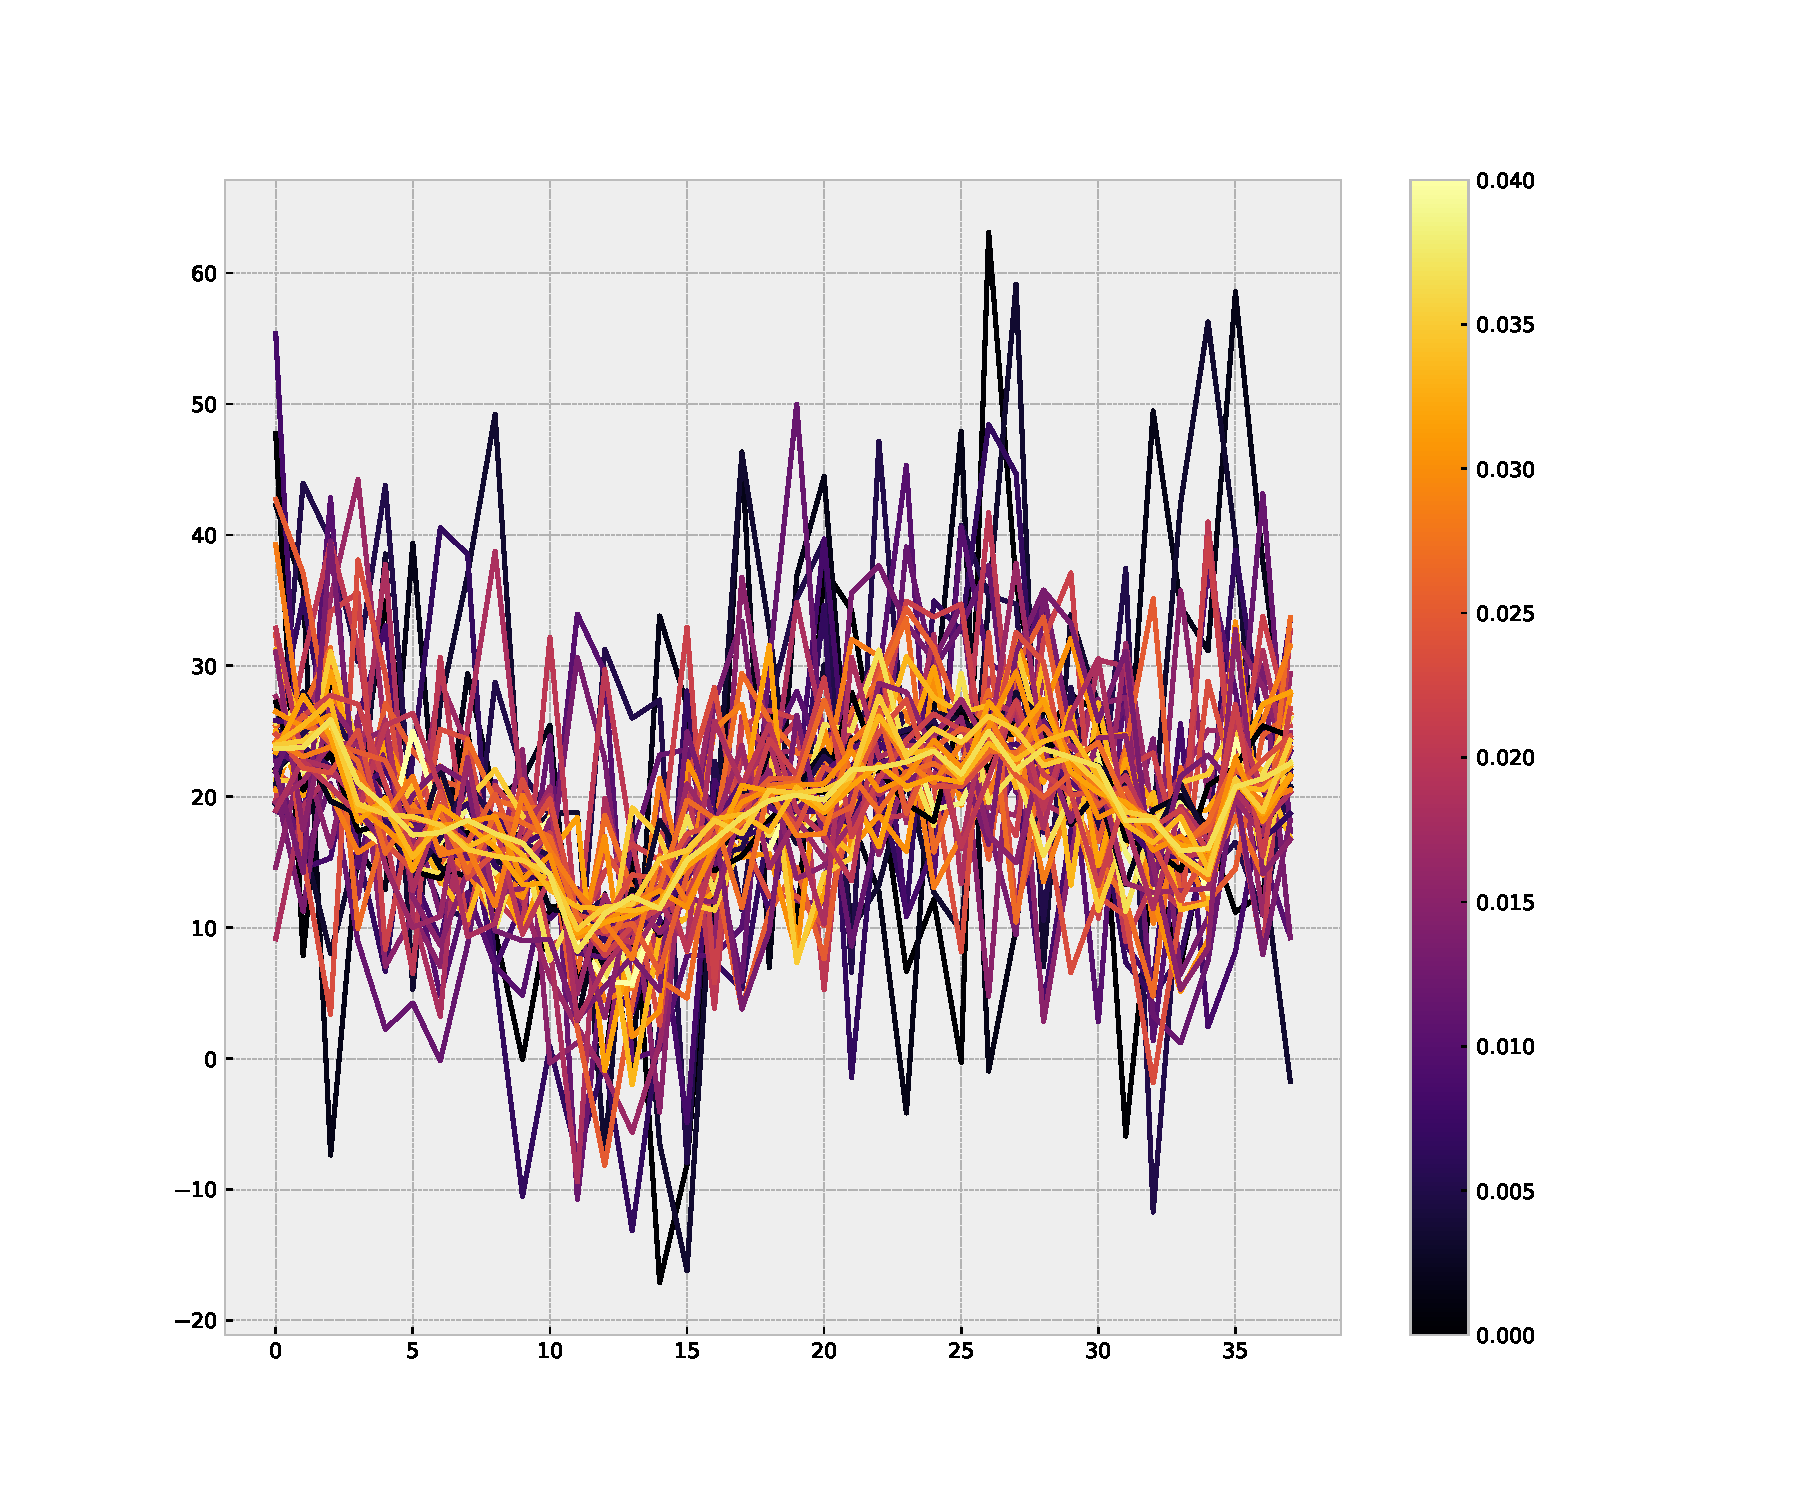
\includegraphics[scale=0.3]{augmentation}
\end{center}
\end{figure}
